\documentclass[twoside]{book}

% Packages required by doxygen
\usepackage{fixltx2e}
\usepackage{calc}
\usepackage{doxygen}
\usepackage[export]{adjustbox} % also loads graphicx
\usepackage{graphicx}
\usepackage[utf8]{inputenc}
\usepackage{makeidx}
\usepackage{multicol}
\usepackage{multirow}
\PassOptionsToPackage{warn}{textcomp}
\usepackage{textcomp}
\usepackage[nointegrals]{wasysym}
\usepackage[table]{xcolor}

% Font selection
\usepackage[T1]{fontenc}
\usepackage[scaled=.90]{helvet}
\usepackage{courier}
\usepackage{amssymb}
\usepackage{sectsty}
\renewcommand{\familydefault}{\sfdefault}
\allsectionsfont{%
  \fontseries{bc}\selectfont%
  \color{darkgray}%
}
\renewcommand{\DoxyLabelFont}{%
  \fontseries{bc}\selectfont%
  \color{darkgray}%
}
\newcommand{\+}{\discretionary{\mbox{\scriptsize$\hookleftarrow$}}{}{}}

% Page & text layout
\usepackage{geometry}
\geometry{%
  a4paper,%
  top=2.5cm,%
  bottom=2.5cm,%
  left=2.5cm,%
  right=2.5cm%
}
\tolerance=750
\hfuzz=15pt
\hbadness=750
\setlength{\emergencystretch}{15pt}
\setlength{\parindent}{0cm}
\setlength{\parskip}{3ex plus 2ex minus 2ex}
\makeatletter
\renewcommand{\paragraph}{%
  \@startsection{paragraph}{4}{0ex}{-1.0ex}{1.0ex}{%
    \normalfont\normalsize\bfseries\SS@parafont%
  }%
}
\renewcommand{\subparagraph}{%
  \@startsection{subparagraph}{5}{0ex}{-1.0ex}{1.0ex}{%
    \normalfont\normalsize\bfseries\SS@subparafont%
  }%
}
\makeatother

% Headers & footers
\usepackage{fancyhdr}
\pagestyle{fancyplain}
\fancyhead[LE]{\fancyplain{}{\bfseries\thepage}}
\fancyhead[CE]{\fancyplain{}{}}
\fancyhead[RE]{\fancyplain{}{\bfseries\leftmark}}
\fancyhead[LO]{\fancyplain{}{\bfseries\rightmark}}
\fancyhead[CO]{\fancyplain{}{}}
\fancyhead[RO]{\fancyplain{}{\bfseries\thepage}}
\fancyfoot[LE]{\fancyplain{}{}}
\fancyfoot[CE]{\fancyplain{}{}}
\fancyfoot[RE]{\fancyplain{}{\bfseries\scriptsize Generated by Doxygen }}
\fancyfoot[LO]{\fancyplain{}{\bfseries\scriptsize Generated by Doxygen }}
\fancyfoot[CO]{\fancyplain{}{}}
\fancyfoot[RO]{\fancyplain{}{}}
\renewcommand{\footrulewidth}{0.4pt}
\renewcommand{\chaptermark}[1]{%
  \markboth{#1}{}%
}
\renewcommand{\sectionmark}[1]{%
  \markright{\thesection\ #1}%
}

% Indices & bibliography
\usepackage{natbib}
\usepackage[titles]{tocloft}
\setcounter{tocdepth}{3}
\setcounter{secnumdepth}{5}
\makeindex

% Hyperlinks (required, but should be loaded last)
\usepackage{ifpdf}
\ifpdf
  \usepackage[pdftex,pagebackref=true]{hyperref}
\else
  \usepackage[ps2pdf,pagebackref=true]{hyperref}
\fi
\hypersetup{%
  colorlinks=true,%
  linkcolor=blue,%
  citecolor=blue,%
  unicode%
}

% Custom commands
\newcommand{\clearemptydoublepage}{%
  \newpage{\pagestyle{empty}\cleardoublepage}%
}

\usepackage{caption}
\captionsetup{labelsep=space,justification=centering,font={bf},singlelinecheck=off,skip=4pt,position=top}

%===== C O N T E N T S =====

\begin{document}

% Titlepage & ToC
\hypersetup{pageanchor=false,
             bookmarksnumbered=true,
             pdfencoding=unicode
            }
\pagenumbering{alph}
\begin{titlepage}
\vspace*{7cm}
\begin{center}%
{\Large Assignment-\/4 }\\
\vspace*{1cm}
{\large Generated by Doxygen 1.8.13}\\
\end{center}
\end{titlepage}
\clearemptydoublepage
\pagenumbering{roman}
\tableofcontents
\clearemptydoublepage
\pagenumbering{arabic}
\hypersetup{pageanchor=true}

%--- Begin generated contents ---
\chapter{Hierarchical Index}
\section{Class Hierarchy}
This inheritance list is sorted roughly, but not completely, alphabetically\+:\begin{DoxyCompactList}
\item Q\+Main\+Window\begin{DoxyCompactList}
\item \contentsline{section}{Dictionary\+Application}{\pageref{classDictionaryApplication}}{}
\end{DoxyCompactList}
\item \contentsline{section}{Word\+Dict}{\pageref{classWordDict}}{}
\item \contentsline{section}{Word\+Trie}{\pageref{classWordTrie}}{}
\end{DoxyCompactList}

\chapter{Class Index}
\doxysection{Class List}
Here are the classes, structs, unions and interfaces with brief descriptions\+:\begin{DoxyCompactList}
\item\contentsline{section}{\mbox{\hyperlink{classBinarySearchTree}{Binary\+Search\+Tree}} }{\pageref{classBinarySearchTree}}{}
\item\contentsline{section}{\mbox{\hyperlink{structnode}{node}} }{\pageref{structnode}}{}
\item\contentsline{section}{\mbox{\hyperlink{classNode}{Node}} }{\pageref{classNode}}{}
\item\contentsline{section}{\mbox{\hyperlink{classRedBlackNode}{Red\+Black\+Node}} }{\pageref{classRedBlackNode}}{}
\item\contentsline{section}{\mbox{\hyperlink{classRedBlackTree}{Red\+Black\+Tree}} }{\pageref{classRedBlackTree}}{}
\end{DoxyCompactList}

\chapter{Class Documentation}
\hypertarget{classDictionaryApplication}{}\section{Dictionary\+Application Class Reference}
\label{classDictionaryApplication}\index{Dictionary\+Application@{Dictionary\+Application}}


Inheritance diagram for Dictionary\+Application\+:\nopagebreak
\begin{figure}[H]
\begin{center}
\leavevmode
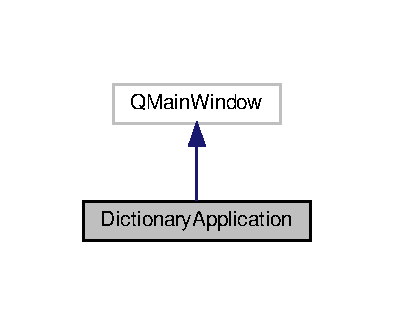
\includegraphics[width=189pt]{classDictionaryApplication__inherit__graph}
\end{center}
\end{figure}


Collaboration diagram for Dictionary\+Application\+:\nopagebreak
\begin{figure}[H]
\begin{center}
\leavevmode
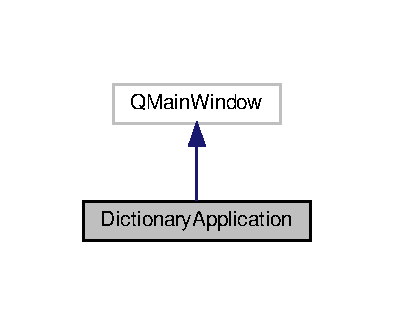
\includegraphics[width=189pt]{classDictionaryApplication__coll__graph}
\end{center}
\end{figure}
\subsection*{Public Member Functions}
\begin{DoxyCompactItemize}
\item 
\mbox{\Hypertarget{classDictionaryApplication_ab56d482375cffd58038600a718329b9b}\label{classDictionaryApplication_ab56d482375cffd58038600a718329b9b}} 
{\bfseries Dictionary\+Application} (Q\+Widget $\ast$parent=nullptr)
\end{DoxyCompactItemize}
\subsection*{Public Attributes}
\begin{DoxyCompactItemize}
\item 
\mbox{\Hypertarget{classDictionaryApplication_aac64e0b0a0c563926f55c7a6e3a3c304}\label{classDictionaryApplication_aac64e0b0a0c563926f55c7a6e3a3c304}} 
Dictionary $\ast$ {\bfseries Word\+Dict}
\end{DoxyCompactItemize}


\subsection{Detailed Description}


Definition at line 10 of file dictionaryapplication.\+h.



The documentation for this class was generated from the following files\+:\begin{DoxyCompactItemize}
\item 
dictionaryapplication.\+h\item 
dictionaryapplication.\+cpp\end{DoxyCompactItemize}

\hypertarget{classWordDict}{}\section{Word\+Dict Class Reference}
\label{classWordDict}\index{Word\+Dict@{Word\+Dict}}


Collaboration diagram for Word\+Dict\+:\nopagebreak
\begin{figure}[H]
\begin{center}
\leavevmode
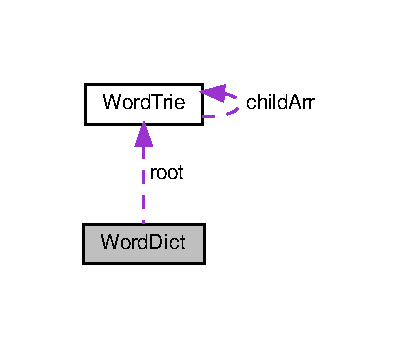
\includegraphics[width=192pt]{classWordDict__coll__graph}
\end{center}
\end{figure}
\subsection*{Public Member Functions}
\begin{DoxyCompactItemize}
\item 
\mbox{\Hypertarget{classWordDict_a8844b0e885a3f390c85bc8439eaeb7eb}\label{classWordDict_a8844b0e885a3f390c85bc8439eaeb7eb}} 
void {\bfseries insert} (string key, string meaning)
\item 
\mbox{\Hypertarget{classWordDict_add3fa0789f86d6c8a791005a84586042}\label{classWordDict_add3fa0789f86d6c8a791005a84586042}} 
string {\bfseries retrieve\+Meaning} (string key)
\item 
\mbox{\Hypertarget{classWordDict_ab5cfeac086dfc61e9928bbe2cbaacf8f}\label{classWordDict_ab5cfeac086dfc61e9928bbe2cbaacf8f}} 
void {\bfseries insert\+\_\+from\+\_\+file} (string filename)
\end{DoxyCompactItemize}
\subsection*{Public Attributes}
\begin{DoxyCompactItemize}
\item 
\mbox{\Hypertarget{classWordDict_a7252f6dc8b8da32689ed39455097e816}\label{classWordDict_a7252f6dc8b8da32689ed39455097e816}} 
\hyperlink{classWordTrie}{Word\+Trie} $\ast$ {\bfseries root}
\end{DoxyCompactItemize}


\subsection{Detailed Description}


Definition at line 53 of file prob1.\+cpp.



The documentation for this class was generated from the following file\+:\begin{DoxyCompactItemize}
\item 
prob1.\+cpp\end{DoxyCompactItemize}

\hypertarget{classWordTrie}{}\section{Word\+Trie Class Reference}
\label{classWordTrie}\index{Word\+Trie@{Word\+Trie}}


Collaboration diagram for Word\+Trie\+:\nopagebreak
\begin{figure}[H]
\begin{center}
\leavevmode
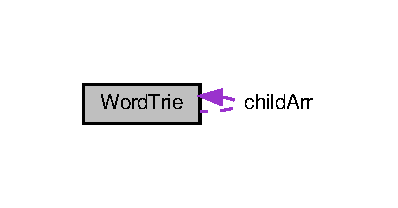
\includegraphics[width=191pt]{classWordTrie__coll__graph}
\end{center}
\end{figure}
\subsection*{Public Member Functions}
\begin{DoxyCompactItemize}
\item 
\mbox{\Hypertarget{classWordTrie_af0cf442ff51c7d278031cec7b3c41a57}\label{classWordTrie_af0cf442ff51c7d278031cec7b3c41a57}} 
\hyperlink{classWordTrie}{Word\+Trie} $\ast$$\ast$ {\bfseries address\+\_\+child} (char character)
\item 
\mbox{\Hypertarget{classWordTrie_a23f941013a4b335793cb58ffe6deb9b4}\label{classWordTrie_a23f941013a4b335793cb58ffe6deb9b4}} 
\hyperlink{classWordTrie}{Word\+Trie} $\ast$ {\bfseries get\+\_\+child\+\_\+with\+\_\+char} (char character)
\end{DoxyCompactItemize}
\subsection*{Public Attributes}
\begin{DoxyCompactItemize}
\item 
\mbox{\Hypertarget{classWordTrie_aa5ec850f660fbe454bfaeb8be355fd51}\label{classWordTrie_aa5ec850f660fbe454bfaeb8be355fd51}} 
bool {\bfseries makes\+\_\+sense}
\item 
\mbox{\Hypertarget{classWordTrie_a2b8ce15c8547d563a0eae5bd3bc0de1a}\label{classWordTrie_a2b8ce15c8547d563a0eae5bd3bc0de1a}} 
string {\bfseries meaning}
\item 
\mbox{\Hypertarget{classWordTrie_a468b4ce929b2348bd59a5fc39a7ecf3f}\label{classWordTrie_a468b4ce929b2348bd59a5fc39a7ecf3f}} 
\hyperlink{classWordTrie}{Word\+Trie} $\ast$ {\bfseries child\+Arr} \mbox{[}26\mbox{]}
\end{DoxyCompactItemize}


\subsection{Detailed Description}


Definition at line 10 of file prob1.\+cpp.



The documentation for this class was generated from the following file\+:\begin{DoxyCompactItemize}
\item 
prob1.\+cpp\end{DoxyCompactItemize}

%--- End generated contents ---

% Index
\backmatter
\newpage
\phantomsection
\clearemptydoublepage
\addcontentsline{toc}{chapter}{Index}
\printindex

\end{document}
